\section{Method}
\label{sec:method}
% =====================================================================

\begin{figure}[t]
  \centering
  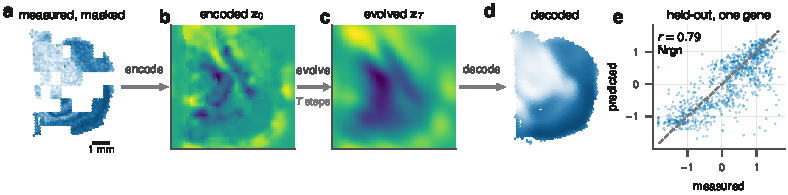
\includegraphics[width=\linewidth]{figures/fig1_overview.pdf}
  \caption{\textbf{Neural Reaction--Diffusion Operator.} Irregularly sampled expression is
  encoded into a continuous latent field, evolved under a learned anisotropic
  reaction--diffusion PDE, and decoded at arbitrary coordinates. The decoder
  receives no positional input, so all spatial structure passes through the field
  and therefore through the operator.}
  \label{fig:overview}
\end{figure}

A section provides $N$ measurements $\{(\vp_i, \vg_i)\}_{i=1}^N$ with positions
$\vp_i \in \R^2$ (isotropically normalized to $[-1,1]^2$) and expression
$\vg_i \in \R^G$. We posit a latent field $\vz : \R^2 \to \R^C$, factored as
encode--evolve--decode.

\paragraph{Spatial encoder.}
Irregular sampling is handled by kernel-integral layers on a $k$-NN graph
\citep{li2020gno}, $\vz_i \leftarrow \sigma( W \vz_i + |\mathcal{N}(i)|^{-1}
\sum_{j\in\mathcal{N}(i)} \kappa_\theta(\vp_j-\vp_i)\odot\vz_j )$, where
$\kappa_\theta$ maps a \emph{relative} displacement to a per-channel gain, so the
layer depends on geometry rather than node identity. Features are splatted onto a
regular $H\times W$ lattice (Nadaraya--Watson, learnable bandwidth), yielding a
field and an \emph{occupancy} map distinguishing ``tissue with no signal'' from
``no measurement here''. Spectral blocks \citep{li2021fno} refine the field.

\paragraph{The reaction--diffusion operator.}
The field evolves under
\begin{equation}
\frac{\partial \vz}{\partial t}
  = \nabla \!\cdot\! \big(\mD_\theta \nabla \vz\big) + f_\theta(\vz),
\label{eq:pde}
\end{equation}
with a per-channel symmetric positive-definite tensor
$\mD_c = L_c L_c^\top + \varepsilon I$ ($L_c$ lower triangular, so definiteness is
structural rather than penalized) and a pointwise reaction network $f_\theta$
implemented as $1\times1$ convolutions with a $\tanh$-bounded output.

Equation~\eqref{eq:pde} is stiff, with diffusion eigenvalues scaling as
$-|\vk|^2$, so an explicit scheme needs $\Delta t = O(h^2/\|\mD\|)$. For
constant-coefficient anisotropic diffusion, however, the operator is diagonal in
the Fourier basis and evolution over $\tau$ has a closed form,
\begin{equation}
E_c(\tau) = \mathcal{F}^{-1}\,
   \exp\!\big(-\vk^\top \mD_c \vk\, \tau\big)\, \mathcal{F} .
\label{eq:expstep}
\end{equation}
Composing \eqref{eq:expstep} with a midpoint reaction update under Strang
splitting \citep{strang1968splitting} yields the one-step map
$S_{\Delta t} = e^{\frac{\Delta t}{2}\mathcal{A}}\circ R_{\Delta t}\circ
e^{\frac{\Delta t}{2}\mathcal{A}}$, which is second-order accurate
(Proposition~\ref{prop:order}). Two structural guarantees follow; both are proved
in Appendix~\ref{app:proofs} and verified numerically in Table~\ref{tab:theory}.

Because $\vk^\top\mD_c\vk\ge0$, the multiplier in \eqref{eq:expstep} lies in
$(0,1]$ for \emph{every} $\Delta t$: the diffusive half-step is an $L^2$
contraction and conserves the spatial mean exactly, with no CFL restriction
(Proposition~\ref{prop:contraction}). Definiteness is structural
($\lambda_{\min}(\mD_c)\ge\varepsilon$), so this holds along the entire
optimization trajectory --- no step size couples to learned parameters and no
projection is required --- and combining it with
$\|f_\theta\|_\infty\le\|g\|_\infty$ yields a uniform absorbing set for the
zero-mean component (Proposition~\ref{prop:bounded}). Section~\ref{sec:numerics}
measures what this buys in practice. The eigenvalues of $\mD_c$ are squared
diffusion lengths per unit pseudo-time, convertible to microns via the stored
coordinate scale.

\paragraph{Decoder.}
Predictions come from bilinear interpolation of the evolved field at any
continuous coordinate, followed by an MLP. \emph{The decoder receives no
positional input}: given coordinates it could memorize a coordinate-to-expression
map, rendering the dynamics ornamental and every ablation uninterpretable.

\paragraph{Objectives.}
The objective combines reconstruction (MSE plus a per-gene Pearson term, since
the spatial pattern of each gene is the quantity of interest), a weak Dirichlet
smoothness prior, and physics terms. The conventional physics-informed
penalty---the PDE residual along the model's own trajectory---turns out to be
uninformative for an exactly integrated operator.

Writing $R_{\Delta t} := \Delta t^{-1}(S_{\Delta t}\vz-\vz) -
(\mathcal{A}_{\mD}\vz+f_\theta(\vz))$, one finds
$\|R_{\Delta t}\| = \tfrac{\Delta t}{2}\|[\mathcal{A}_{\mD},\mathcal{F}_\theta]\vz\|
+ O(\Delta t^2)$ uniformly over bounded parameter sets, with no dependence on the
observations (Proposition~\ref{prop:vacuity}). Minimizing $\|R_{\Delta t}\|^2$
therefore cannot fit the model to data---the data do not appear---and merely
biases $\theta$ toward operators whose diffusive and reactive parts commute
(Appendix~\ref{app:vacuity}). We instead impose the
constraint that the \emph{measured configuration be a near-stationary state} of
the learned operator,
\begin{equation}
\mathcal{L}_{\mathrm{PDE}} = \big\| \nabla\!\cdot\!(\mD_\theta \nabla \vz_T)
  + f_\theta(\vz_T) \big\|^2 ,
\label{eq:steady}
\end{equation}
the natural formalization of the quasi-steady-state assumption for adult tissue,
which constrains $\mD_\theta$ and $f_\theta$ jointly. Mass, Jacobian-norm and
splitting-consistency terms are also included.

\paragraph{Interpretability.}
Linearizing \eqref{eq:pde} about a homogeneous $\vz^*$ gives $\partial_t
\delta\vz_{\vk} = (\mJ - \vk^\top\!\mD\vk)\,\delta\vz_{\vk}$ with $\mJ =
\nabla f_\theta(\vz^*)$, so $\max\mathrm{Re}\,\mathrm{spec}(\mJ - |\vk|^2\mD)$
against $|\vk|$ is the dispersion relation of the learned operator --- a
falsifiable read-out of the dynamics it has inferred (Appendix~\ref{app:turing}).

% =====================================================================
